\documentclass[10pt,a4paper,twoside,onecolumn]{article}

% Use UTF-8 for plain tex files
\usepackage[utf8]{inputenc}

% Set the margin from the page side
\usepackage[margin=3cm]{geometry}

% Leave out page numbers on empty pages
\let\origdoublepage\cleardoublepage
\renewcommand{\cleardoublepage}{%
  \clearpage
  {\pagestyle{empty}\origdoublepage}%
}

% Don't indent paragrpahs, instead separate them
\usepackage{parskip}
\setlength{\parskip}{5mm plus2mm minus3mm}
\setlength{\parindent}{0cm}

% Use alternative font (see http://www.tug.dk/FontCatalogue/ for alternatives)
\usepackage{cmbright}
\renewcommand*\familydefault{\sfdefault} % Set the default font to be sans-serif
\linespread{1.05}         % Palatino needs more leading (space between lines)
\usepackage[T1]{fontenc}

% Allow URL typesetting
\usepackage{url}

% Customize headers and footers
\usepackage{fancyhdr}

% Includegraphics support
\usepackage{graphicx}

% Allows to change text color
\usepackage{color}
\usepackage[usenames,dvipsnames]{xcolor}

% Assign the LastPage label to the last page
\usepackage{lastpage}

% TODO: Add description
\usepackage{hyperref}

% Enable the creation of appendices
\usepackage{appendix}

% Set layout lenghts
\setlength{\headheight}{8mm}
\setlength{\footskip}{1.5cm}
\addtolength{\textheight}{-.5cm}

% Set titles whitespace
\usepackage{titlesec}
\titlespacing{\section}{0mm}{8mm}{1mm}
\titlespacing{\subsection}{0mm}{3mm}{-2mm}
\titlespacing{\subsubsection}{0mm}{2mm}{-1mm}

% Miscellaneous
\definecolor{mselogogray}{RGB}{96,101,109} % Color definition for the MSE logo


\settitle{Lab. 05 – Network Information}{Certified IT Security}
\addauthor{Julien Oberson}
\addauthor{Jonathan Stoppani}

\input{headers-footers}


%-----------------------------------------------------------------------------
% Use special numbering and formatting to match the questions numbering in the
% workbook document
\usepackage{chngcntr}

% First question is #16
\setcounter{section}{15}

% Questions are broken down by different listings
\def\thesubsection{Listing \arabic{subsection}:}

% Single questions are numbered using letters
\def\thesubsubsection{\alph{subsubsection})}

% Single questions numbering is identical for whole global questions
\counterwithout*{subsubsection}{subsection}
\counterwithin*{subsubsection}{section}

% Adapt spacing in the TOC to account for numbering scheme
\setlength\cftsubsubsecnumwidth{1.5em}
\setlength\cftsubsecnumwidth{4.1em}
%-----------------------------------------------------------------------------


\begin{document}

	\title{Certified IT Secuirty\\  Lab. 01 -- Port scan}
\author{Julien Oberson \and Jonathan Stoppani}

\begin{titlepage}
\thispagestyle{empty}

\vspace*{10mm}
\includegraphics{images/logo_mse}
\vspace{5mm}

\hrule
\vspace{0.2mm}
{\Large Certified IT Security}\\[2mm]
{\Huge Lab. 01 -- Port scan}\\[1mm]
\hrule

\begin{minipage}[t]{0.5\textwidth}
    \begin{flushleft}
        Julien \textsc{Oberson}\\
        Jonathan \textsc{Stoppani}
    \end{flushleft}
\end{minipage}
\begin{minipage}[t]{0.495\textwidth}
	\begin{flushright}
        \today
	\end{flushright}
\end{minipage}

\vfill

\tableofcontents

\end{titlepage}


	\content

	\section{Mail headers analysis}


\subsection{Mail headers dump}


\subsubsection{Identity and organization of the sender}

The two mail were sent by Marta (using the address \email{marta@salleurl.edu}) and Rick (using the address \email{rick@salleurl.edu}), respectively. The organization to which they belong to is the \emph{La Salle Ramon Llull University} as can be inferred from the domain of their email addressese: \texttt{salleurl.edu}.

In the case of Rick, the \texttt{X-Authentication-Warning} header suggests that the content of the \texttt{From} header could have been forged (but probably wasn't, for the reasons described at the following URL: \url{http://www.slingcode.com/pineauthenticationwarning.php}).


\subsubsection{Mail clients used to send the messages}

Marta is probably using Microsoft Outlook Express, version 6.00.2800.1158 to send their emails as shwon in the \texttt{X-Mailer} header. In Rick's case, no \texttt{X-Mailer} header is provided, but the combination of the information provided by the \texttt{X-Authentication-Warning} and \texttt{Message-ID} headers almost certainly indicate that the mail was sent using Pine\footnote{Pine is a tool for reading, sending and managing emails, developed by UW Technology at the University of Washington: \url{http://www.washington.edu/pine/}.}.

It is worth to note that the headers which were used to retrieve this information can easily be forged by the message sender and they could thus report incorrect data.


\subsubsection{Network addresses}

The different network addresses extracted from the email headers are: \texttt{10.0.14.198}, \texttt{130.206.42.238} and \texttt{130.206.42.246} for the email sent by Marta to Pete and \texttt{127.0.0.1} (the not that useful loopback address), \texttt{130.206.42.238} and \texttt{130.206.42.246} for the email from Rick to Pete.

A communication diagram for the two email which also includes the IP addresses of the involved parties, is represented in the Figure~\vref{fig:mail}.


\subsubsection{Network software and versions}

The network softwares used by the involved parties are \texttt{sendmail} (used by the LaSalle University network) and \texttt{qmail} (used by Pete's email provider).

It is possible to retrieve \texttt{sendmail}'s version by analyzing the headers: \texttt{columba.salleurl.edu} is running version {\tt 8.12.9} while \texttt{relay1.salleurl.edu} is running version {\tt 8.12.8p1}. Additionally, in the second email transaction, \texttt{sendmail} also exposes the underlying operating system for \texttt{columba.salleurl.edu}: \texttt{Debian 3}.

As already seen in the preceding answer, network software and versions are also included in the communication diagram \vpageref{fig:mail}.


\subsubsection{Domains}

As done with the IP addresses, domains can also easily be extracted from the email headers. The already cited {\tt columba.salleurl.edu} and {\tt relay1.salleurl.edu}; the originating server for the first email: {\tt LEGOLAS}; and Pete's email provider: {\tt fithwor.pair.com} were found. The two email domains {\tt salleurl.edu} and {\tt isecom.org} can also be listed here.

Together with the IP addresses and the newtork softwares, domains are also shown in the Figure~\vref{fig:mail}.

\begin{figure}[p]
	\centering

	\subfloat[fig:marta-pete][Email from marta to pete]{
		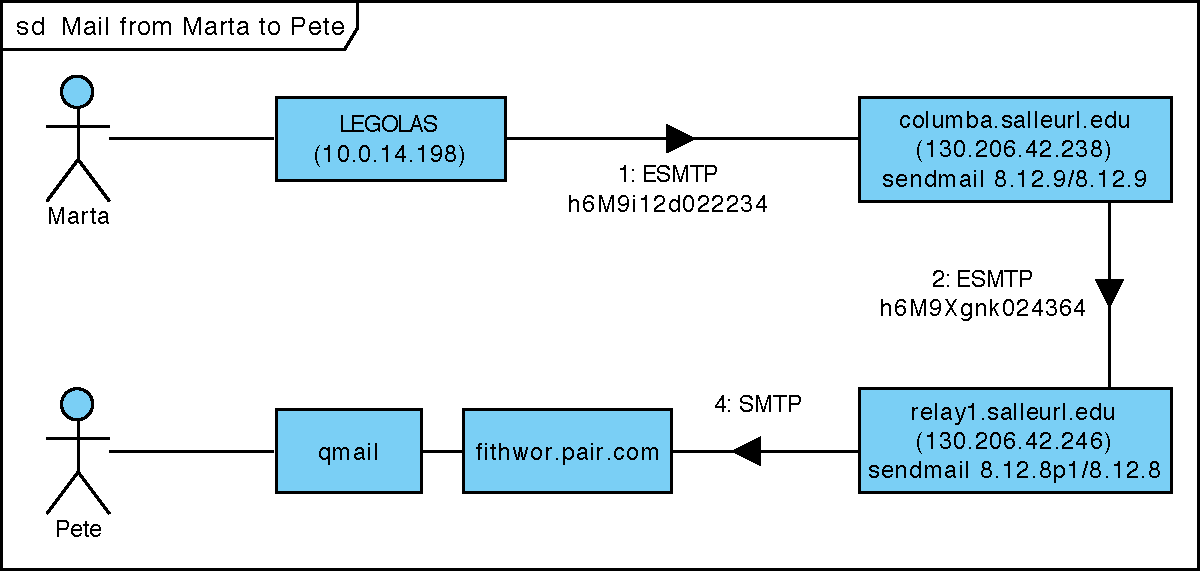
\includegraphics[scale=0.5]{uml/marta-pete}
	}
	\\[10mm]

	\subfloat[fig:rick-pete][Email from Rick to Pete]{
		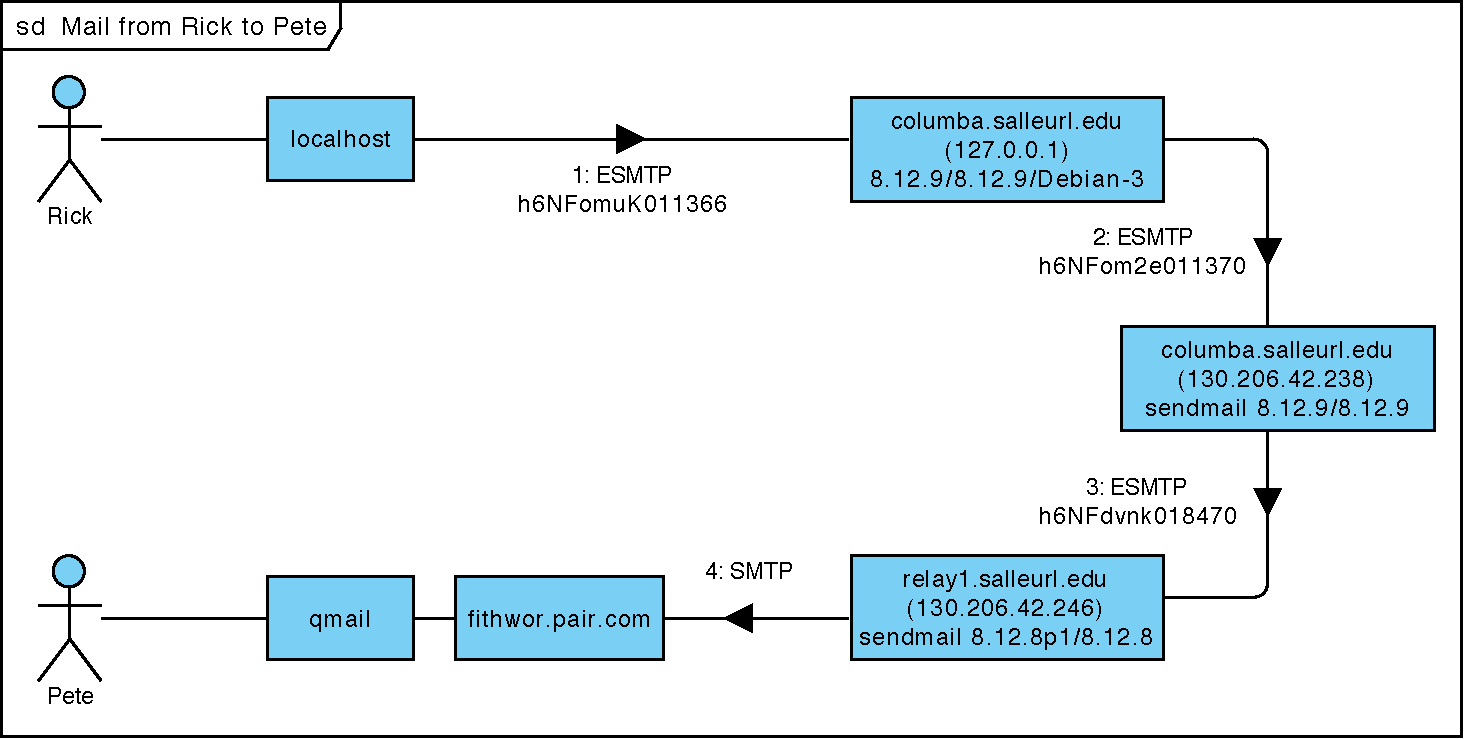
\includegraphics[scale=0.5]{uml/rick-pete}
	}
	\\[5mm]

	\caption{Communication diagrams for the different hosts intervening in the mail transmission between the three actors.}
	\label{fig:mail}
\end{figure}

	\section{HTTP headers analysis}

\subsection{\texttt{302 Moved Temporarily} response}

\subsubsection{Reasons for the 302 error}
TODO

\subsubsection{Changes between HTTP/1.0 and HTTP/1.1}
TODO



\subsection{\texttt{200 OK} response}

\subsubsection{Type of the server}

As indicated by the {\tt Server} response header, the server runs {\tt Apache} version {\tt 1.3.27}.

\subsubsection{Determination of virtual hosting}
TODO



\subsection{\texttt{OPTIONS} request}

\subsubsection{Request type and information}

The request is an {\tt OPTIONS} request. The HTTP/1.1 specifications describes this request type as:

\begin{quote}
The OPTIONS method represents a request for information about the communication options available on the request/response chain identified by the Request-URI. This method allows the client to determine the options and/or requirements associated with a resource, or the capabilities of a server, without implying a resource action or initiating a resource retrieval.
\end{quote}

In this specific case, the webserver itself does accept all request types defined by HTTP/1.1, namely: {\tt GET}, {\tt POST}, {\tt HEAD}, {\tt PUT}, {\tt DELETE}, {\tt CONNECT}, {\tt OPTIONS} and {\tt TRACE} (including the {\tt PATCH} extension). Additionally, the {\tt PROPFIND}, {\tt PROPPATCH}, {\tt MKCOL}, {\tt COPY}, {\tt MOVE}, {\tt LOCK} and {\tt UNLOCK} WebDAV methods are also supported.

\subsubsection{Discovered weaknesses}

By including the WebDAV methods in the reply, the server exposes its WebDAV handling capabilities. If WebDAV access isn't properly protected through the use of authentication and authorization, this can led to public access to the website and, in a worse-case scenario, to other important assets stored on the server.



\subsection{\texttt{GET} request with \texttt{REFERRER}}

\subsubsection{Server type}

The returned server type is a custom Rapidsite\footnote{Rapidsite is an hostig provider registered in the United States: \url{http://www.rapidsite.net/}} branded version of {\tt Apache} (version {\tt 1.3.27}) running on some flavor of Unix. Additionally, the FrontPage extensions (version {\tt 5.0.2.2510}) and the SSL module (version {\tt 2.8.12} with {\tt OpenSSL} version {\tt 0.9.7a}) are installed.

\subsubsection{Determination of virtual hosting for www.isecom.info}
TODO

\subsubsection{Discovered weaknesses}

The installed FrontPage server extensions are a serious security risk if not correctly configured as they allow remote files uploading and expose dynamic components to be used insite web pages (such as counters, server-side image maps, search forms,...).

Considered the {\tt ETag} timestamp (June 2003), {\tt Apache/1.3.28} was just released and {\tt OpenSSL} was not yet outdated; the installed software does not pose thus a security risk. If, instead, we consider the current date (April, 2010) and the current versions of the software used by Rapidsite\footnote{A rapid check revelead that Rapidsite is still using outdated packages: {\tt Apache/1.3.33}, the same {\tt FrontPage} server extensions and {\tt OpenSSL/0.9.8d} (released in September 2006).}, there is an urgent need to upgrade the whole server software stack.



\subsection{\texttt{GET} request with blank \texttt{HOST}}

\subsubsection{Information inferred from the test}
TODO

\subsubsection{Changes to be made to extract more information}
TODO

	\section{Network registration analysis}

\subsection{\texttt{dyadsecurity.com} network registration}

\subsubsection{Domain name registrar}

This domain was registered through GoDaddy.

\subsubsection{Duration of domain purchase}

The domain was purchased for the duration of one year (Jan. 19, 2003 --- Jan. 19, 2004).

\subsubsection{Document grinding information}

The different exposed contact information could be used for document grinding purposes as full names, addresses and contact information are exposed. In this specific case, the following information can be extracted:

\begin{quote}
\textit{Robert Lee\\
Dyad Security, Inc.\\
3400 Irving Ave., Bldg 118\\
Newport Beach, California 92660\\
United States}\\
\\
Phone: \textit{(949) 486-6600}\\
Email: \textit{registration@dyadsecurity.com}
\end{quote}



\subsection{\texttt{zc.tv} network registration}

\subsubsection{Domain name registrar}

No information about the domain name registrar was found in the provided information.

\subsubsection{Duration of domain purchase}

The domain was purchased for the duration of three years (Nov. 27, 2000 --- Nov. 27, 2003).

\subsubsection{Document grinding information}

As seen above for the {\tt dyadsecurity.com} domain registration information, also for {\tt zc.tv} the same principle applies. In this specific case, the following information can be extracted:

\begin{minipage}[t]{0.5\textwidth}
	\begin{quote}
		\textit{%
			William Graham\\
			Zoom Culture\\
			10005 Main St.\\
			Chapel Hill, NC 27516\\
			United States
		}\\
		\\
		Phone: \textit{(919) 960-9512}\\
		Email: \textit{bill@zoomculture.com}
	\end{quote}
\end{minipage}
\begin{minipage}[t]{0.5\textwidth}
	\begin{quote}
		\textit{%
			Nathan Wieler\\
			Zoom Culture\\
			10005 Main St.\\
			Chapel Hill, NC 27516\\
			United States
		}\\
		\\
		Phone: \textit{(919) 960-9512}\\
		Email: \textit{nate@salesmaninc.com}
	\end{quote}
\end{minipage}

	\section{DNS queries analysis}

\subsection{\texttt{salleurl.edu} DNS request}

\subsubsection{Primary name server}

TODO: Is it possible to say for sure the the primary is aries? Or is it not yet known which one is the primary one?

The primary name server for the {\tt salleurl.edu} domain is {\tt aries.salleurl.edu}. Two additional name servers are also available, namely {\tt relay1.salleurl.edu} and {\tt relay2.salleurl.edu}.

\subsubsection{Extracted domains and IP addresses}

The {\tt salleurl.edu} domain binds to the IP address {\tt 130.206.42.160}.

Three additional hostnames (the three DNS servers presented in the preceding answer) were also discovered. Their IPs are {\tt 130.206.42.224}, {\tt 130.206.42.224} and {\tt 130.206.42.123} for {\tt aries.}, {\tt relay1.} and {\tt relay2.salleurl.edu}, respectively.

\subsubsection{Purpose of the test}

TODO: ???



\subsection{\texttt{salleurl.edu} authoritative DNS request}

\subsubsection{Primary name server}

The primary name server for the {\tt salleurl.edu} domain is {\tt aries.salleurl.edu}, as clearly indicated by the {\tt MNAME} field of the {\tt SOA} record.

\subsubsection{Extracted domains and IP addresses}

Beside the name servers and the root domain already presented in the previous answer, this test revelaed one more hostname: {\tt columba.salleurl.edu} with the IP address {\tt 130.206.42.238}. Additionally, the four {\tt MX} records state that all of {\tt aries.}, {\tt relay1.}, {\tt relay2.} and {\tt columba.salleurl.edu} are also mail exchange servers.

\subsubsection{Purpose of the test}

The purpose of this test is to retrieve all DNS information (using the {\tt any} flag) for the {\tt salleurl.edu} domain by interrogating the primary name server ({\tt aries.salleurl.edu}) directly and obtaining thus an authoritative answer.



\subsection{\texttt{salleurl.edu} complete DNS listing}

\subsubsection{Purpose of the test}

The prupose of this test is to execute a zone transfer for the {\tt salleurl.edu} domain from one of its name servers. A zone transfer would allow the requester to retrieve all the DNS information for the {\tt salleurl.edu} domain stored on the queried name server.

\subsubsection{Test results}

All three tested name servers ({\tt aries.}, {\tt relay1.} and {\tt relay2.salleurl.edu}) denied the zone transfer and revelead no additional information.


	\appendix

	\section{References and external resources}

\begin{itemize}
	\item Common Internet Message Headers\\\url{http://www.ietf.org/rfc/rfc2076.txt}
	\item Standard for the format of ARPA Internet text messages\\\url{http://www.ietf.org/rfc/rfc0822.txt}
	\item Requirements for Internet Hosts -- Application and Support\\\url{http://www.ietf.org/rfc/rfc1123.txt}
	\item What does ``invoked from network'' means?\\\url{http://www.gossamer-threads.com/lists/qmail/users/17790}
	\item Hypertext Transfer Protocol -- HTTP/1.1: Method definitions\\\url{http://www.w3.org/Protocols/rfc2616/rfc2616-sec9.html}
	\item PATCH Method for HTTP\\\url{http://tools.ietf.org/html/rfc5789}
	\item HTTP Extensions for Distributed Authoring -- WEBDAV\\\url{http://www.ietf.org/rfc/rfc2518.txt}
	\item FrontPage Server Extensions\\\url{http://en.wikipedia.org/wiki/FrontPage_Server_Extensions}
	\item Domain names -- Implementation and specification\\\url{http://tools.ietf.org/html/rfc1035}
\end{itemize}


\end{document}
